% LaTeX Template: Project Titlepage Modified (v 0.1) by rcx
%
% Original Source: http://www.howtotex.com
% Date: February 2014
% 
% This is a title page template which be used for articles & reports.
% 
% This is the modified version of the original Latex template from
% aforementioned website.

\documentclass[12pt]{article}
\usepackage[a4paper]{geometry}
\usepackage[myheadings]{fullpage}
\usepackage{fancyhdr}
\usepackage{lastpage}
\usepackage{graphicx, wrapfig, setspace, booktabs}
\usepackage[T1]{fontenc}
\usepackage[font=small, labelfont=bf]{caption}
\usepackage{fourier}
\usepackage[protrusion=true, expansion=true]{microtype}
\usepackage[english]{babel}
\usepackage{sectsty}
\usepackage{url, lipsum}
\usepackage{tgbonum}
\usepackage{hyperref}
\usepackage{xcolor}
\usepackage{enumerate}
\usepackage{listings}
\usepackage{lstautogobble}
\usepackage{subfigure}

\newcommand{\HRule}[1]{\rule{\linewidth}{#1}}
\onehalfspacing
\setcounter{tocdepth}{5}
\setcounter{secnumdepth}{5}



%-------------------------------------------------------------------------------
% HEADER & FOOTER
%-------------------------------------------------------------------------------
\pagestyle{fancy}
\fancyhf{}
\setlength\headheight{15pt}
\fancyhead[L]{Student ID: 10406141}
\fancyhead[R]{University of Manchester}
\fancyfoot[R]{Page \thepage\ of \pageref{LastPage}}
%-------------------------------------------------------------------------------
% TITLE PAGE
%-------------------------------------------------------------------------------

\begin{document}
{\fontfamily{cmr}\selectfont
\title{ \normalsize \textsc{}
		\\ [2.0cm]
		\HRule{0.5pt} \\
		\LARGE \textbf{\uppercase{Lab3 Report}
		\HRule{2pt} \\ [0.5cm]
		\normalsize \today \vspace*{5\baselineskip}}
		}

\date{}

\author{
		Wenchang Liu \\ 
		ID: 10406141 \\
		School of Computer Science }

\maketitle
\newpage
\tableofcontents
\newpage

%-------------------------------------------------------------------------------
% Section title formatting
\sectionfont{\scshape}
%-------------------------------------------------------------------------------

%-------------------------------------------------------------------------------
% BODY
%-------------------------------------------------------------------------------

\section{Ex1 Lexical Analysis}
\label{sec: ex1}
\begin{enumerate}[1.]
	\item POS tag the sentence

	Sentence: Steel is an alloy of iron and carbon, and sometimes other elements. 
	Because of its high tensile strength and low cost, it is a major component used in buildings, 
	infrastructure, tools, ships, automobiles, machines, appliances, and weapons.

	Steel(NNP) is(VBZ) an(DT) alloy(NN) of(IN) iron(NN) and(CC) carbon(NN) ,(,) and(CC) sometimes(RB) 
	other(JJ) elements(NNS) .(.) Because(IN) of(IN) its(PRP\$) high(JJ) tensile(NN) strength(NN) and(CC) 
	low(JJ) cost(NN) ,(,) it(PRP) is(VBZ) a(DT) major(JJ) component(NN) used(VBN) in(IN) buildings(NNS) ,(,) 
	infrastructure(NN) ,(,) tools(NNS) ,(,) ships(NNS) ,(,) automobiles(NNS) ,(,) machines(NNS) ,(,) 
	appliances(NNS) ,(,) and(CC) weapons(NNS) .(.)

	\item Identify the pronominal co-references

	Co-references are "its" and "it".

\end{enumerate}

\newpage
\section{Ex2 C-Structures}
\label{sec: ex2}
\begin{enumerate}[1.]
	\item Plot the constituency (phrase) structure: 
		Sentence: ‘Steel is an alloy of iron and carbon, and sometimes other elements’.
		\begin{figure}[ht]
			\centering
			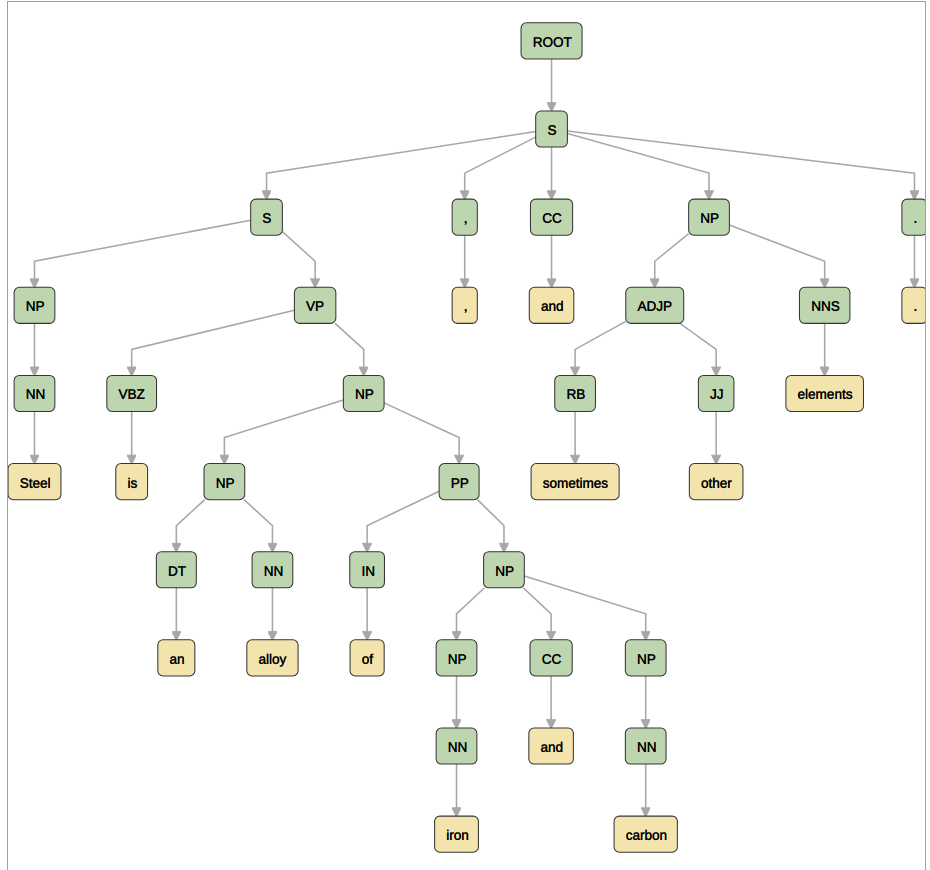
\includegraphics[scale=0.3]{figs/constituency_parse.png}
			\caption{Constituency Parse Plot}
			\label{fig:label}
		\end{figure}
	\item List the nominal phrasal nodes (NPs) correspond to ‘molecules of meaning’ for that sentence

		NP: Steel, an alloy, iron, carbon, iron and carbon, an alloy of iron and carbon, sometimes other elements.
	\item List the coordinations within that sentence.

		CC: and(iron and carbon), and(and sometimes other elements)
\end{enumerate}

\newpage
\section{Ex3 Dependencies - Exploring new territories}
\label{sec: ex3}
\begin{enumerate}[1.]
	\item What is the difference between dependency and constituency? 
	
	Dependency parsing: A dependency parse connects words according to their relationships. 
	Each vertex in the tree represents a word, child nodes are words that are dependent on the parent, 
	and edges are labeled by the relationship.
	
	Constituency parsing: A constituency parse tree breaks a text into sub-phrases. 
	Non-terminals in the tree are types of phrases, the terminals are the words in the sentence, 
	and the edges are unlabeled.
	\item What is emphasised by each representation?
	
	Dependency parsing: Emphasising the dependency relationships between words.

	Constituency parsing: Emphasising sub-phrases within the sentence.
	\item Draw the dependency structure of the following sentence: ‘Steel is analloy of iron and carbon’.
	
	nsubj: nominal subject

	cop: copula

	det: determiner

	nmod: nominal modifier

	case: prepositions, postpositions and other case markers

	cc: coordinating conjunction

	conj: conjunct

	\begin{figure}[ht]
		\centering
		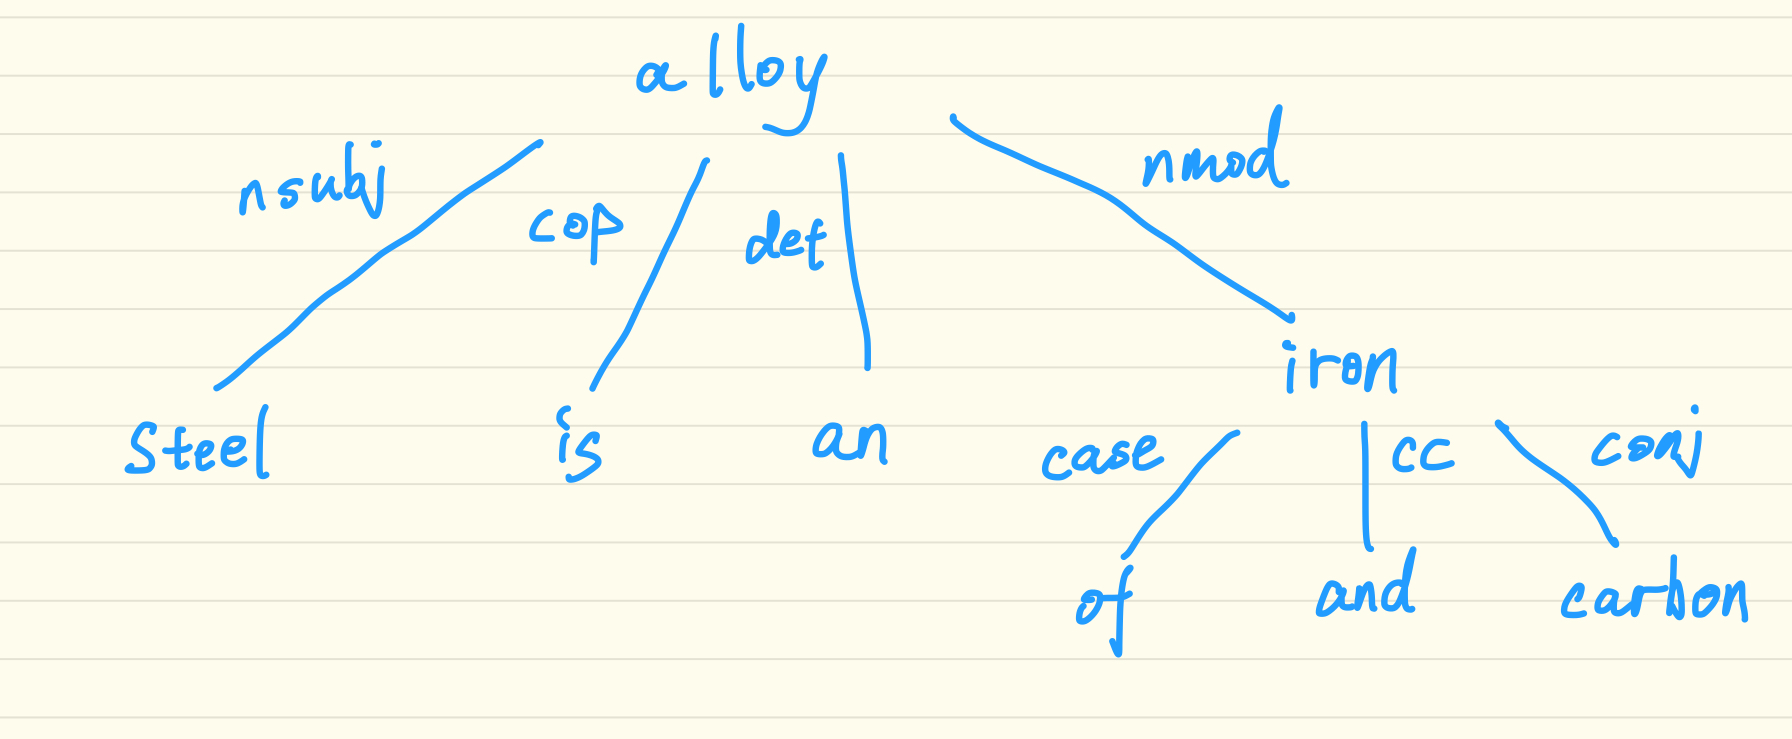
\includegraphics[scale=0.2]{figs/dependency_parse.jpg}
		\caption{Dependency Parse Structure}
		\label{fig:label1}
	\end{figure}

\end{enumerate}

\newpage
\section{Ex4 OpenIE - Semantics}
\label{sec: ex4}
\begin{enumerate}[1.]
	\item Use openIE to extract the predicate-argument structure of:
	\begin{enumerate}[(1)]
		\item "Steel is an alloy":
		\begin{figure}[ht]
			\centering
			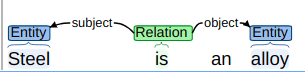
\includegraphics[scale=0.45]{figs/Openie1.png}
			\caption{OpenIE result for 'Steel is an alloy'}
			\label{fig:label2}
		\end{figure}
		\item "Steel contains carbon":
		\begin{figure}[ht]
			\centering
			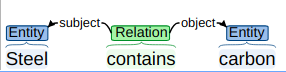
\includegraphics[scale=0.45]{figs/Openie2.png}
			\caption{OpenIE result for 'Steel contains carbon'}
			\label{fig:label3}
		\end{figure}
		\item "Steel contains iron":
		\begin{figure}[ht]
			\centering
			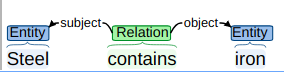
\includegraphics[scale=0.45]{figs/Openie3.png}
			\caption{OpenIE result for 'Steel contains iron'}
			\label{fig:label4}
		\end{figure}
	\end{enumerate}
	\item Represent the triples above using Prolog:
	\begin{lstlisting}
		alloy(X) :- steel(X).
		containsCarbon(X) :- steel(X).
		containsIron(X) :- steel(X).
	\end{lstlisting}
	\item Represent the triples above using RDF:
	\begin{lstlisting}
		<Steel> <is an> <alloy>.
		<Steel> <contains> <carbon>.
		<Steel> <contains> <iron>.
	\end{lstlisting}
	\item Formalise the axioms using Description Logics:
	\begin{center}
	$Steel \sqsubseteq Alloy$

	$Steel \rightarrow \exists Contain.Carbon$

	$Steel \rightarrow \exists Contain.Iron$
	\end{center}
	\item Analyse what happens when getting "Steel is an alloy of iron and carbon.":
	
	There are two relations in terms of "Steel"(subject), one is relation "is" (i.e. Steel is an alloy), 
	the other is relation "an alloy of" (i.e. Steel 'is an alloy of' iron), and the objects are "alloy" 
	and "iron" respectively.
	\begin{figure}[ht]
		\centering
		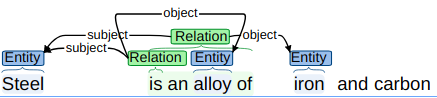
\includegraphics[scale=0.45]{figs/Openie4.png}
		\caption{OpenIE result for 'Steel is an alloy of iron and carbon'}
		\label{fig:label5}
	\end{figure}
\end{enumerate}

\newpage
\section{Ex5 Complex OpenIE, Rhetorical Structures}
\label{sec: ex5}

Sentence: 'As the carbon percentage content rises, steel has the ability to become harder 
and stronger through heat treating; however, it becomes less ductile.'
\begin{enumerate}[1.]
	\item Identify the nucleus and the satellites
	
	nucleus: "however, it becomes less ductile."

	satellites: "As the carbon percentage content rises, steel has the ability to become harder 
	and stronger through heat treating;"
	\item Draw the diagram with the rhetorical relations
	\begin{figure}[ht]
		\centering
		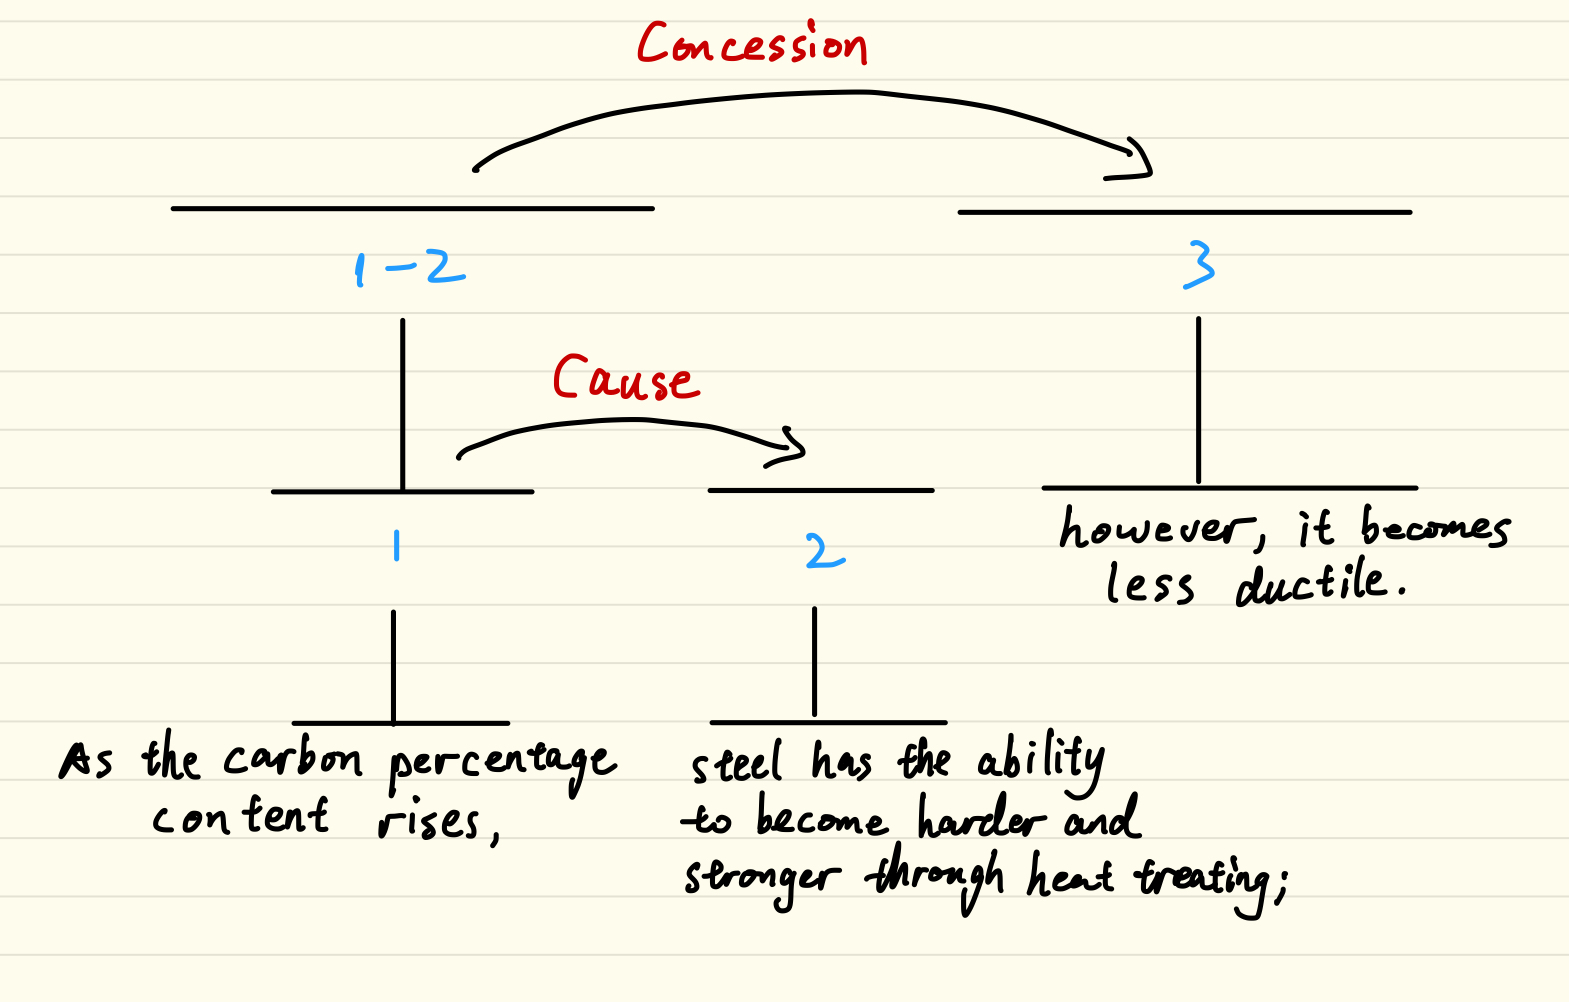
\includegraphics[scale=0.15]{figs/rhetorical_structure.jpg}
		\caption{rhetorical relation diagram}
		\label{fig:label6}
	\end{figure}
	\item Which relations are hypotactic or paratactic?
	
	The "concession" and "cause" are both hypotactic.
	\item Write the output for that sentence using the RDF-NL notation of Graphene
	\begin{figure}[ht]
		\centering
		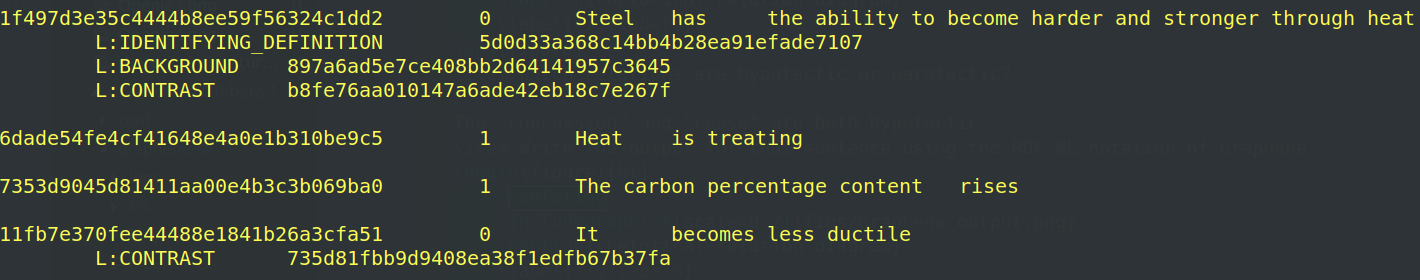
\includegraphics[scale=0.3]{figs/Graphene_output.png}
		\caption{output from Graphene}
		\label{fig:label7}
	\end{figure}
	
\end{enumerate}

\newpage
\section{Ex6 Taxonomies, Thesauri}
\label{sec: ex6}
\begin{enumerate}[1.]
	\item List the WordNet glosses for 'martensite' and 'austenite'
	
	martensite: a solid solution of carbon in alpha-iron that is formed when steel is cooled so rapidly that 
	the change from austenite to pearlite is suppressed; responsible for the hardness of quenched steel.

	austenite: a solid solution of ferric carbide or carbon in iron; cools to form pearlite or martensite.
	\item List the Taxonomic/Hypernym chain up to the top for these two terms
	
	martensite/austenite -> solid solution, primary solid solution -> solution -> mixture -> substance ->

	(1) matter -> physical entity -> entity

	(2) part, portion, component part, component, constituent -> relation -> abstraction, abstract entity -> entity

	\item List their sibling terms: 
	ferrite, double salt
	\item For the word 'temper': 
	\begin{enumerate}[(1)]
		\item how many synsets do we have? 9 synsets. 
		\item Which senses are related to steel? 
			\begin{enumerate}[1*]
				\item the elasticity and hardness of a metal object; 
				its ability to absorb considerable energy before cracking
				\item bring to a desired consistency, texture, or hardness by a process of gradually heating and cooling
				\item harden by reheating and cooling in oil
			\end{enumerate}
		\item What are its synonyms? (n)toughness; (v)anneal, normalize; (v)harden
		\item Would you consider these perfect or near-synonyms? 
		
		For anneal and normalize, I think they are perfect, but for toughness and harden, they are near-synonyms. 
		Because for anneal and normalize, they are very specific and mean exactly the same thing, but for toughness, 
		I think it is more a similar meaning not exactly the same.
	\end{enumerate}
\end{enumerate}

\newpage
\section{Ex7 Frame Semantics - Exploring Further}
\label{sec: ex7}
\begin{enumerate}[1.]
	\item Describe the frame semantics for "melt" "oxidize" as listed by VerbNet, Prop-Bank and FrameNet
	\begin{enumerate}[(1)]
		\item VerbNet:
		
			$melt: KNEAD-26.5, OTHER\_COS-45.4-1$

			$oxidize: ENTITY\_SPECIFIC\_COS-45.5, OTHER\_COS-45.4$
		\item Prop-Bank: 
		
			$melt: MELT.v$

			$oxidize: OXIDIZE.v$
		\item FrameNet:
		
			$melt: CAUSE\_CHANGE\_OF\_PHASE, CHANGE\_OF\_PHASE$

			$oxidize: CORRODING\_CAUSED$
	\end{enumerate}
	\item How these representations compare?
	
	Prop-Bank is tightly connected to VerbNet lexicon, and can increase verb coverage, it 
	is made by generalized semantic roles, defined as prototypes and has fewer thematic roles 
	compared to FrameNet, which define roles specific to a group of predicates.
	\item Using the FrameNet semantics, draw the Conceptual Graph for the following sentence:  
	‘At 1433 degrees, the material started to progressively melt around the edges.’
	\begin{figure}[ht]
		\centering
		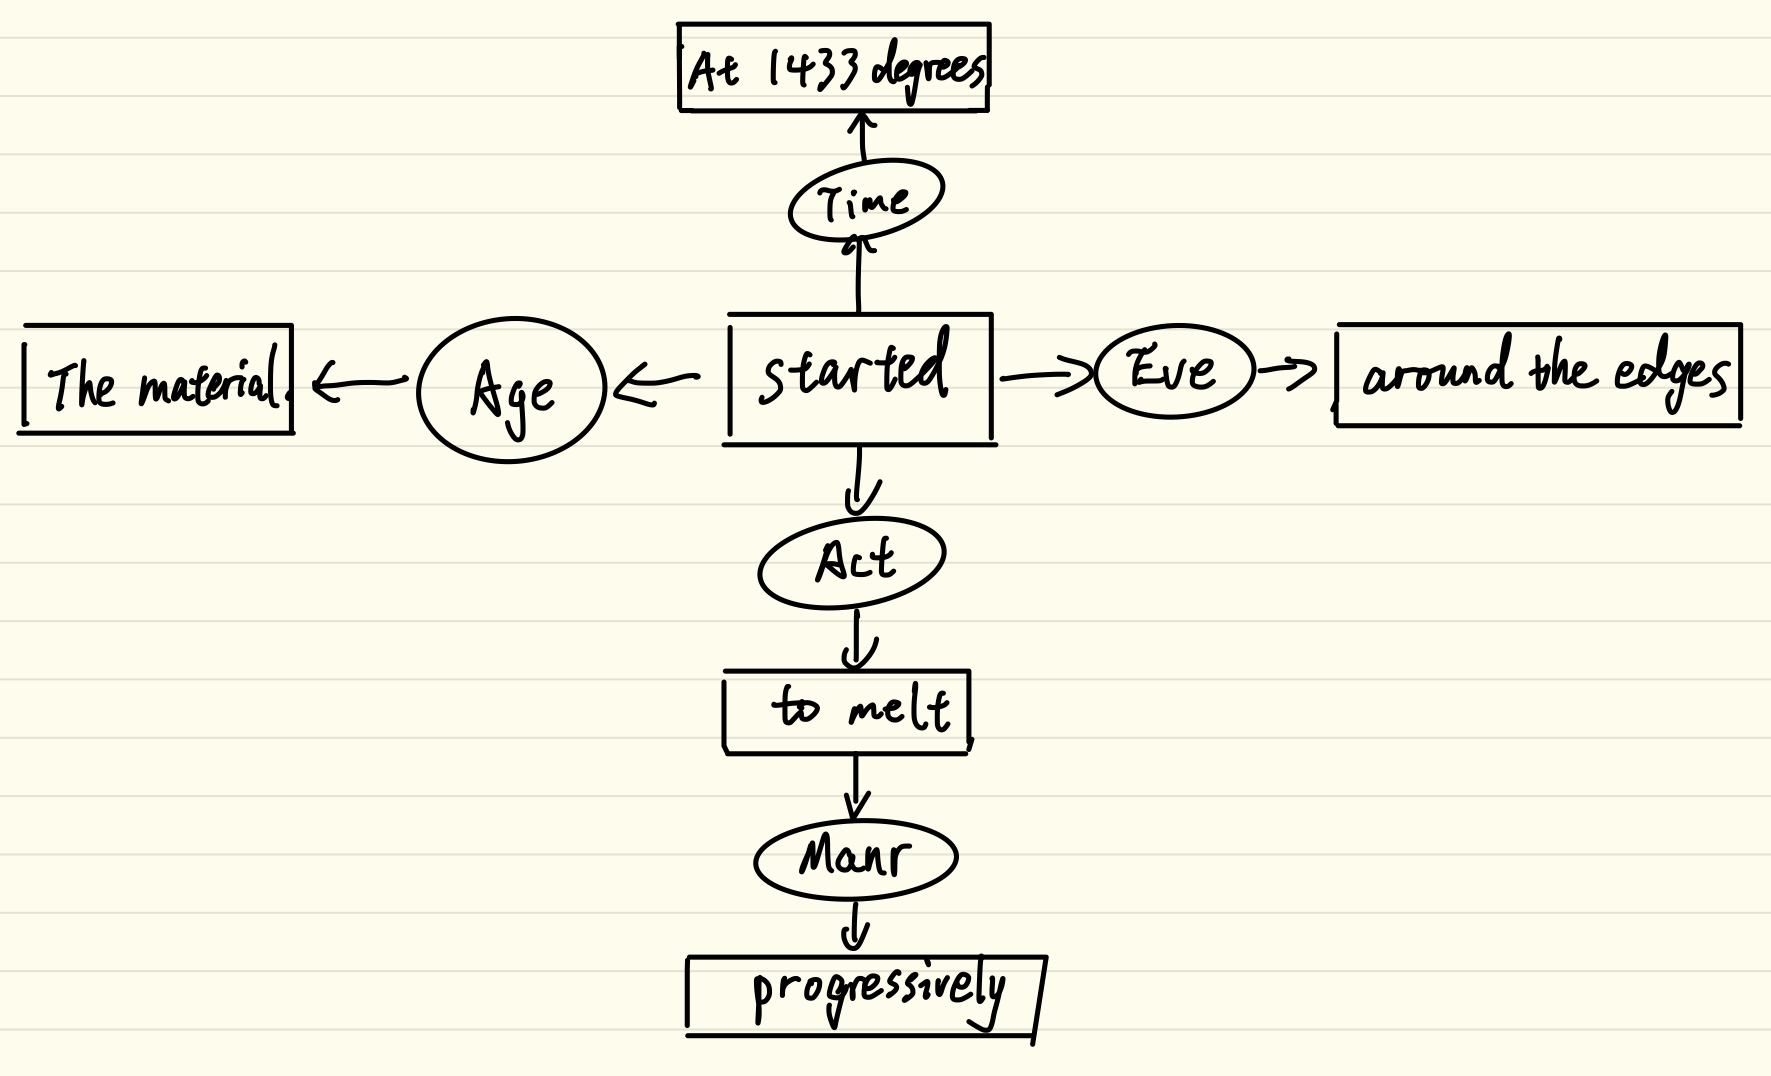
\includegraphics[scale=0.18]{figs/conceptual_graph.jpg}
		\caption{Conceptual graph for the sentence}
		\label{fig:label8}
	\end{figure}
\end{enumerate}

\newpage
\section{Ex8 Ontologies - Description Logics}
\label{sec: ex8}
Ex8: Convert the natural language statements into an ontology.

Here are some screenshots of the work:
\begin{figure}[ht]
	\centering
	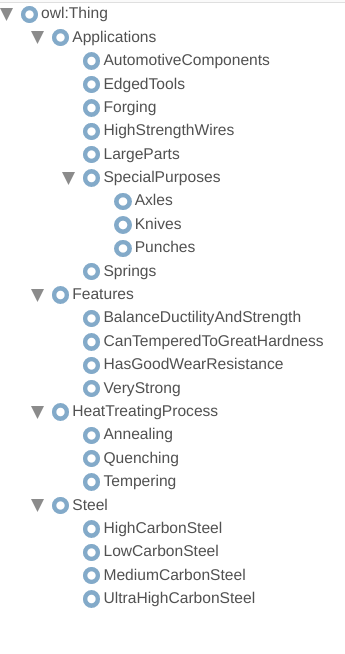
\includegraphics[scale=0.4]{figs/ex8-class-hierarchy.png}
	\caption{Class hierarchy of the ontology}
	\label{fig:label9}
\end{figure}
\begin{figure}[ht]
	\centering
	\subfigure[object property]{
		\begin{minipage}{7cm}
			\centering
			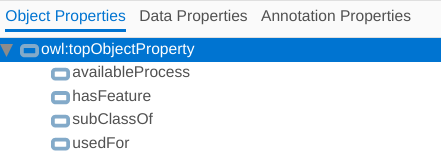
\includegraphics[scale=0.25]{figs/ex8-object-properties.png}
		\end{minipage}
	}
	\subfigure[data property]{
		\begin{minipage}{7cm}
			\centering
			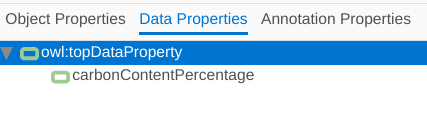
\includegraphics[scale=0.25]{figs/ex8-data-property.png}
		\end{minipage}
	}
	\caption{Properties}
	\label{fig:label10}
\end{figure}
\begin{figure}[ht]
	\centering
	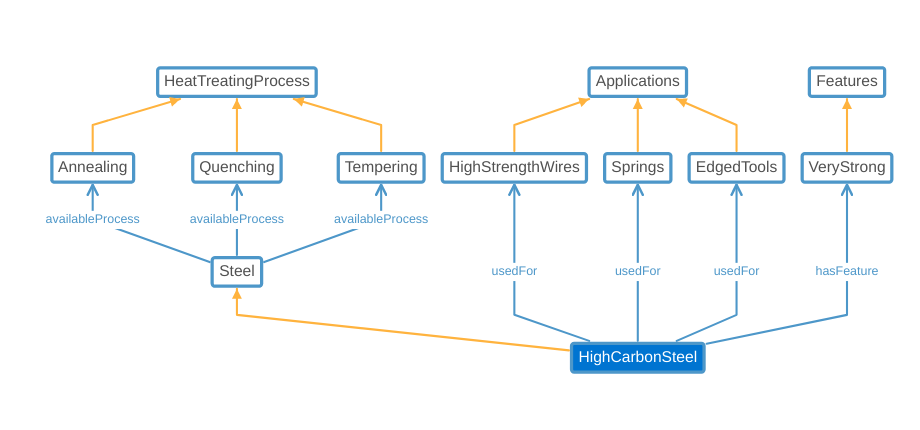
\includegraphics[scale=0.3]{figs/ex8-highcarbonsteel-example.png}
	\caption{an example entity graph of high carbon steel}
	\label{fig:label11}
\end{figure}

See OWL file for more details in appendix A.

\section{Ex9 Inductive \& Deductive Reasoning}
\label{sec: ex9}
\begin{enumerate}[1.]
	\item Using ILP to learn the definitions of each type of crystallographic structure
	
	FERRITE(X, Y) <- MEDIUMTEMPERATURE(X), LOWCARBON(Y).
	
	PEARLITE(X,Y) <- LOWTEMPERATURE(X), MEDIUMCARBON(Y).
	
	AUSTENITE(X,Y) <- MEDIUMTEMPERATURE(X), MEDIUMCARBON(Y).
	
	CEMENTITE(X,Y) <- MEDIUMTEMPERATURE(X), HIGHCARBON(Y).
	\item Perform deductive reasoning:
	
	Are the materials solid or liquid?
	
	All of theses materials are solid.

	\begin{figure}[ht]
		\centering
		\subfigure[ferrite]{
			\begin{minipage}{7cm}
				\centering
				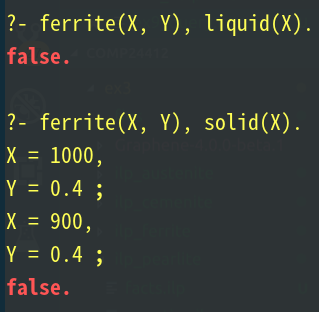
\includegraphics[scale=0.35]{figs/ex9-2-1.png}
			\end{minipage}
		}
		\subfigure[pearlite]{
			\begin{minipage}{7cm}
				\centering
				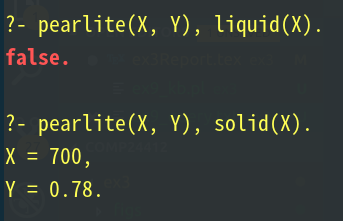
\includegraphics[scale=0.35]{figs/ex9-2-2.png}
			\end{minipage}
		}
		\subfigure[austenite]{
			\begin{minipage}{7cm}
				\centering
				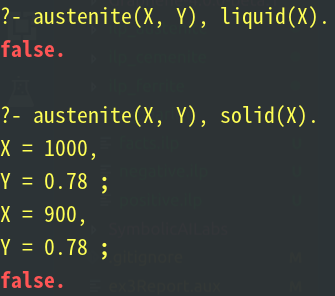
\includegraphics[scale=0.35]{figs/ex9-2-3.png}
			\end{minipage}
		}
		\subfigure[cementite]{
			\begin{minipage}{7cm}
				\centering
				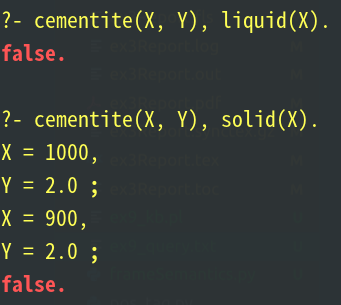
\includegraphics[scale=0.35]{figs/ex9-2-4.png}
			\end{minipage}
		}
		\caption{Query: are materials solid or liquid}
		\label{fig:label12}
	\end{figure}

	\item Deductive again:
	
	Does Ferrite have high hardness? Why?

	No. There is no carbon content that can fit both ferrite and high hardness.

	\begin{figure}[ht]
		\centering
		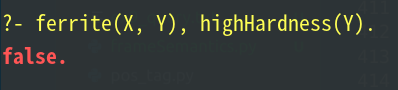
\includegraphics[scale=0.3]{figs/ex9-3-1.png}
		\caption{Query: does ferrite have high hardness}
		\label{fig:label13}
	\end{figure}

	Is Ferrite more ductile than Cementite? Why?

	Yes. Ferrite is high ductility but cementite is not.

	\begin{figure}[ht]
		\centering
		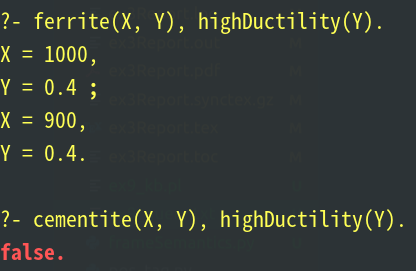
\includegraphics[scale=0.3]{figs/ex9-3-2.png}
		\caption{Query: is ferrite more ductile than cementite}
		\label{fig:label14}
	\end{figure}

	Which material has low tensile strength? Why?

	Ferrite. Only ferrtie's carbon content can fit low tensile strength.

	\begin{figure}[ht]
		\centering
		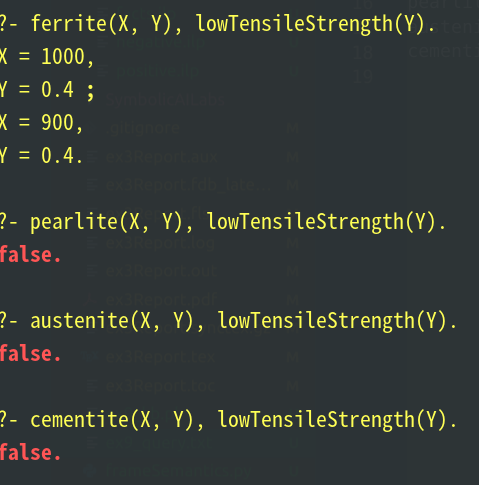
\includegraphics[scale=0.3]{figs/ex9-3-3.png}
		\caption{Query: which material has low tensile strength}
		\label{fig:label15}
	\end{figure}

\end{enumerate}

\newpage
\section{Appendix A: Ontology XML}
\label{sec: AppendixA}
\lstset{basicstyle=\tiny}
\begin{lstlisting}
<?xml version="1.0"?>
<Ontology xmlns="http://www.w3.org/2002/07/owl#"
		xml:base="http://webprotege.stanford.edu/project/DxITv9MAicsSUu54ZOu2qG"
		xmlns:rdf="http://www.w3.org/1999/02/22-rdf-syntax-ns#"
		xmlns:xml="http://www.w3.org/XML/1998/namespace"
		xmlns:xsd="http://www.w3.org/2001/XMLSchema#"
		xmlns:rdfs="http://www.w3.org/2000/01/rdf-schema#"
		ontologyIRI="http://webprotege.stanford.edu/project/DxITv9MAicsSUu54ZOu2qG">
	<Prefix name="owl" IRI="http://www.w3.org/2002/07/owl#"/>
	<Prefix name="rdf" IRI="http://www.w3.org/1999/02/22-rdf-syntax-ns#"/>
	<Prefix name="xml" IRI="http://www.w3.org/XML/1998/namespace"/>
	<Prefix name="xsd" IRI="http://www.w3.org/2001/XMLSchema#"/>
	<Prefix name="rdfs" IRI="http://www.w3.org/2000/01/rdf-schema#"/>
	<Declaration>
		<Class IRI="http://webprotege.stanford.edu/R77HrYnkWf8yOdwxl3WuW1A"/>
	</Declaration>
	<Declaration>
		<Class IRI="http://webprotege.stanford.edu/R7AO81oJArvkzcjwXCtd4FC"/>
	</Declaration>
	<Declaration>
		<Class IRI="http://webprotege.stanford.edu/R7SKPSPclcU0G2HYHr94Ysk"/>
	</Declaration>
	<Declaration>
		<Class IRI="http://webprotege.stanford.edu/R7Wt4ZAjowWum6jGTa6cfv4"/>
	</Declaration>
	<Declaration>
		<Class IRI="http://webprotege.stanford.edu/R7k56fVzJcAkhFQaIEkYFSv"/>
	</Declaration>
	<Declaration>
		<Class IRI="http://webprotege.stanford.edu/R7rzlu1B3N23vhiIi73jGdI"/>
	</Declaration>
	<Declaration>
		<Class IRI="http://webprotege.stanford.edu/R846GMVxIMEtXgXybWAhIyh"/>
	</Declaration>
	<Declaration>
		<Class IRI="http://webprotege.stanford.edu/R8Ej3tVsjP5Tujpp2onZ3Vj"/>
	</Declaration>
	<Declaration>
		<Class IRI="http://webprotege.stanford.edu/R8SgCQGCUPS4cPRItcYai2T"/>
	</Declaration>
	<Declaration>
		<Class IRI="http://webprotege.stanford.edu/R97OWwnTdiaAcIuIL6AKjTU"/>
	</Declaration>
	<Declaration>
		<Class IRI="http://webprotege.stanford.edu/R9H1s0evsYMcedUicerleF"/>
	</Declaration>
	<Declaration>
		<Class IRI="http://webprotege.stanford.edu/R9yy7Q58I36dWTaomJ0AXE8"/>
	</Declaration>
	<Declaration>
		<Class IRI="http://webprotege.stanford.edu/RB5l4cXsOisMbebzSFwcIS9"/>
	</Declaration>
	<Declaration>
		<Class IRI="http://webprotege.stanford.edu/RBeeFtU5HwRSVJ9WO3x4ttl"/>
	</Declaration>
	<Declaration>
		<Class IRI="http://webprotege.stanford.edu/RCMNXtsT7lXkcYrxO6nbnf8"/>
	</Declaration>
	<Declaration>
		<Class IRI="http://webprotege.stanford.edu/RCp1BzKb6cmUuQCt9gBiIsq"/>
	</Declaration>
	<Declaration>
		<Class IRI="http://webprotege.stanford.edu/RCtWKPeM4CphKE6VdL4d97v"/>
	</Declaration>
	<Declaration>
		<Class IRI="http://webprotege.stanford.edu/RDQQlz564YgakVQW2SiPU1N"/>
	</Declaration>
	<Declaration>
		<Class IRI="http://webprotege.stanford.edu/RDRRjjmED0zPvkyeU7TcN4G"/>
	</Declaration>
	<Declaration>
		<Class IRI="http://webprotege.stanford.edu/RDRaSF2IL8pbEI59iTgzNsi"/>
	</Declaration>
	<Declaration>
		<Class IRI="http://webprotege.stanford.edu/RDWA3v5bJVW3VQoVRoM7zX8"/>
	</Declaration>
	<Declaration>
		<Class IRI="http://webprotege.stanford.edu/RDe1Cs54n6wUTMYYNavFMuQ"/>
	</Declaration>
	<Declaration>
		<Class IRI="http://webprotege.stanford.edu/RZFYpU9e4GSQcvFxNExtlR"/>
	</Declaration>
	<Declaration>
		<Class IRI="http://webprotege.stanford.edu/RnpAm5YZIAcl4mr9ZbfPJy"/>
	</Declaration>
	<Declaration>
		<Class IRI="http://webprotege.stanford.edu/RzLMMM8OeWX5JtMmZdpFwD"/>
	</Declaration>
	<Declaration>
		<ObjectProperty IRI="http://webprotege.stanford.edu/R9NHcdNpt6OdcTPXR2AuszN"/>
	</Declaration>
	<Declaration>
		<ObjectProperty IRI="http://webprotege.stanford.edu/RBxTDEpGv7sSa7xJNtZ18C6"/>
	</Declaration>
	<Declaration>
		<ObjectProperty IRI="http://webprotege.stanford.edu/RG8xtrhT3IRlly1RC1A2I3"/>
	</Declaration>
	<Declaration>
		<ObjectProperty IRI="http://webprotege.stanford.edu/RjSaLrVf3vINT3S6d3vWkn"/>
	</Declaration>
	<Declaration>
		<DataProperty IRI="http://webprotege.stanford.edu/RmF9qJDswdWG6qQ4xfUPyQ"/>
	</Declaration>
	<Declaration>
		<NamedIndividual IRI="http://webprotege.stanford.edu/R7aYMvvsLZak4GJXeegSHo8"/>
	</Declaration>
	<Declaration>
		<Datatype IRI="http://webprotege.stanford.edu/R8VZPAaOyVnkvotw6Wr3HOc"/>
	</Declaration>
	<SubClassOf>
		<Class IRI="http://webprotege.stanford.edu/R77HrYnkWf8yOdwxl3WuW1A"/>
		<Class IRI="http://webprotege.stanford.edu/RDe1Cs54n6wUTMYYNavFMuQ"/>
	</SubClassOf>
	<SubClassOf>
		<Class IRI="http://webprotege.stanford.edu/R7AO81oJArvkzcjwXCtd4FC"/>
		<Class IRI="http://webprotege.stanford.edu/RCMNXtsT7lXkcYrxO6nbnf8"/>
	</SubClassOf>
	<SubClassOf>
		<Class IRI="http://webprotege.stanford.edu/R7AO81oJArvkzcjwXCtd4FC"/>
		<DataHasValue>
			<DataProperty IRI="http://webprotege.stanford.edu/RmF9qJDswdWG6qQ4xfUPyQ"/>
			<Literal xml:lang="en">float[&gt;=&quot;0.05&quot;, &lt;=&quot;0.30&quot;]</Literal>
		</DataHasValue>
	</SubClassOf>
	<SubClassOf>
		<Class IRI="http://webprotege.stanford.edu/R7SKPSPclcU0G2HYHr94Ysk"/>
		<Class IRI="http://webprotege.stanford.edu/R9yy7Q58I36dWTaomJ0AXE8"/>
	</SubClassOf>
	<SubClassOf>
		<Class IRI="http://webprotege.stanford.edu/R7Wt4ZAjowWum6jGTa6cfv4"/>
		<Class IRI="http://webprotege.stanford.edu/RCMNXtsT7lXkcYrxO6nbnf8"/>
	</SubClassOf>
	<SubClassOf>
		<Class IRI="http://webprotege.stanford.edu/R7Wt4ZAjowWum6jGTa6cfv4"/>
		<ObjectSomeValuesFrom>
			<ObjectProperty IRI="http://webprotege.stanford.edu/RBxTDEpGv7sSa7xJNtZ18C6"/>
			<Class IRI="http://webprotege.stanford.edu/R8Ej3tVsjP5Tujpp2onZ3Vj"/>
		</ObjectSomeValuesFrom>
	</SubClassOf>
	<SubClassOf>
		<Class IRI="http://webprotege.stanford.edu/R7Wt4ZAjowWum6jGTa6cfv4"/>
		<ObjectSomeValuesFrom>
			<ObjectProperty IRI="http://webprotege.stanford.edu/RG8xtrhT3IRlly1RC1A2I3"/>
			<Class IRI="http://webprotege.stanford.edu/RDRRjjmED0zPvkyeU7TcN4G"/>
		</ObjectSomeValuesFrom>
	</SubClassOf>
	<SubClassOf>
		<Class IRI="http://webprotege.stanford.edu/R7Wt4ZAjowWum6jGTa6cfv4"/>
		<DataHasValue>
			<DataProperty IRI="http://webprotege.stanford.edu/RmF9qJDswdWG6qQ4xfUPyQ"/>
			<Literal>float[&gt;=&quot;1.25&quot;, &lt;=&quot;2.0&quot;]</Literal>
		</DataHasValue>
	</SubClassOf>
	<SubClassOf>
		<Class IRI="http://webprotege.stanford.edu/R7k56fVzJcAkhFQaIEkYFSv"/>
		<Class IRI="http://webprotege.stanford.edu/R9yy7Q58I36dWTaomJ0AXE8"/>
	</SubClassOf>
	<SubClassOf>
		<Class IRI="http://webprotege.stanford.edu/R7rzlu1B3N23vhiIi73jGdI"/>
		<Class IRI="http://webprotege.stanford.edu/R8Ej3tVsjP5Tujpp2onZ3Vj"/>
	</SubClassOf>
	<SubClassOf>
		<Class IRI="http://webprotege.stanford.edu/R846GMVxIMEtXgXybWAhIyh"/>
		<Class IRI="http://webprotege.stanford.edu/RCMNXtsT7lXkcYrxO6nbnf8"/>
	</SubClassOf>
	<SubClassOf>
		<Class IRI="http://webprotege.stanford.edu/R846GMVxIMEtXgXybWAhIyh"/>
		<ObjectSomeValuesFrom>
			<ObjectProperty IRI="http://webprotege.stanford.edu/RBxTDEpGv7sSa7xJNtZ18C6"/>
			<Class IRI="http://webprotege.stanford.edu/R7k56fVzJcAkhFQaIEkYFSv"/>
		</ObjectSomeValuesFrom>
	</SubClassOf>
	<SubClassOf>
		<Class IRI="http://webprotege.stanford.edu/R846GMVxIMEtXgXybWAhIyh"/>
		<ObjectSomeValuesFrom>
			<ObjectProperty IRI="http://webprotege.stanford.edu/RBxTDEpGv7sSa7xJNtZ18C6"/>
			<Class IRI="http://webprotege.stanford.edu/RCtWKPeM4CphKE6VdL4d97v"/>
		</ObjectSomeValuesFrom>
	</SubClassOf>
	<SubClassOf>
		<Class IRI="http://webprotege.stanford.edu/R846GMVxIMEtXgXybWAhIyh"/>
		<ObjectSomeValuesFrom>
			<ObjectProperty IRI="http://webprotege.stanford.edu/RBxTDEpGv7sSa7xJNtZ18C6"/>
			<Class IRI="http://webprotege.stanford.edu/RZFYpU9e4GSQcvFxNExtlR"/>
		</ObjectSomeValuesFrom>
	</SubClassOf>
	<SubClassOf>
		<Class IRI="http://webprotege.stanford.edu/R846GMVxIMEtXgXybWAhIyh"/>
		<ObjectSomeValuesFrom>
			<ObjectProperty IRI="http://webprotege.stanford.edu/RG8xtrhT3IRlly1RC1A2I3"/>
			<Class IRI="http://webprotege.stanford.edu/RB5l4cXsOisMbebzSFwcIS9"/>
		</ObjectSomeValuesFrom>
	</SubClassOf>
	<SubClassOf>
		<Class IRI="http://webprotege.stanford.edu/R846GMVxIMEtXgXybWAhIyh"/>
		<ObjectSomeValuesFrom>
			<ObjectProperty IRI="http://webprotege.stanford.edu/RG8xtrhT3IRlly1RC1A2I3"/>
			<Class IRI="http://webprotege.stanford.edu/RBeeFtU5HwRSVJ9WO3x4ttl"/>
		</ObjectSomeValuesFrom>
	</SubClassOf>
	<SubClassOf>
		<Class IRI="http://webprotege.stanford.edu/R846GMVxIMEtXgXybWAhIyh"/>
		<DataHasValue>
			<DataProperty IRI="http://webprotege.stanford.edu/RmF9qJDswdWG6qQ4xfUPyQ"/>
			<Literal xml:lang="en">float[&gt;=&quot;0.3&quot;, &lt;=&quot;0.6&quot;]</Literal>
		</DataHasValue>
	</SubClassOf>
	<SubClassOf>
		<Class IRI="http://webprotege.stanford.edu/R8Ej3tVsjP5Tujpp2onZ3Vj"/>
		<Class IRI="http://webprotege.stanford.edu/R9yy7Q58I36dWTaomJ0AXE8"/>
	</SubClassOf>
	<SubClassOf>
		<Class IRI="http://webprotege.stanford.edu/R8SgCQGCUPS4cPRItcYai2T"/>
		<Class IRI="http://webprotege.stanford.edu/R8Ej3tVsjP5Tujpp2onZ3Vj"/>
	</SubClassOf>
	<SubClassOf>
		<Class IRI="http://webprotege.stanford.edu/R97OWwnTdiaAcIuIL6AKjTU"/>
		<Class IRI="http://webprotege.stanford.edu/R8Ej3tVsjP5Tujpp2onZ3Vj"/>
	</SubClassOf>
	<SubClassOf>
		<Class IRI="http://webprotege.stanford.edu/R9H1s0evsYMcedUicerleF"/>
		<Class IRI="http://webprotege.stanford.edu/R9yy7Q58I36dWTaomJ0AXE8"/>
	</SubClassOf>
	<SubClassOf>
		<Class IRI="http://webprotege.stanford.edu/RB5l4cXsOisMbebzSFwcIS9"/>
		<Class IRI="http://webprotege.stanford.edu/RCp1BzKb6cmUuQCt9gBiIsq"/>
	</SubClassOf>
	<SubClassOf>
		<Class IRI="http://webprotege.stanford.edu/RBeeFtU5HwRSVJ9WO3x4ttl"/>
		<Class IRI="http://webprotege.stanford.edu/RCp1BzKb6cmUuQCt9gBiIsq"/>
	</SubClassOf>
	<SubClassOf>
		<Class IRI="http://webprotege.stanford.edu/RCMNXtsT7lXkcYrxO6nbnf8"/>
		<ObjectSomeValuesFrom>
			<ObjectProperty IRI="http://webprotege.stanford.edu/RjSaLrVf3vINT3S6d3vWkn"/>
			<Class IRI="http://webprotege.stanford.edu/R77HrYnkWf8yOdwxl3WuW1A"/>
		</ObjectSomeValuesFrom>
	</SubClassOf>
	<SubClassOf>
		<Class IRI="http://webprotege.stanford.edu/RCMNXtsT7lXkcYrxO6nbnf8"/>
		<ObjectSomeValuesFrom>
			<ObjectProperty IRI="http://webprotege.stanford.edu/RjSaLrVf3vINT3S6d3vWkn"/>
			<Class IRI="http://webprotege.stanford.edu/RDRaSF2IL8pbEI59iTgzNsi"/>
		</ObjectSomeValuesFrom>
	</SubClassOf>
	<SubClassOf>
		<Class IRI="http://webprotege.stanford.edu/RCMNXtsT7lXkcYrxO6nbnf8"/>
		<ObjectSomeValuesFrom>
			<ObjectProperty IRI="http://webprotege.stanford.edu/RjSaLrVf3vINT3S6d3vWkn"/>
			<Class IRI="http://webprotege.stanford.edu/RzLMMM8OeWX5JtMmZdpFwD"/>
		</ObjectSomeValuesFrom>
	</SubClassOf>
	<SubClassOf>
		<Class IRI="http://webprotege.stanford.edu/RCtWKPeM4CphKE6VdL4d97v"/>
		<Class IRI="http://webprotege.stanford.edu/R9yy7Q58I36dWTaomJ0AXE8"/>
	</SubClassOf>
	<SubClassOf>
		<Class IRI="http://webprotege.stanford.edu/RDQQlz564YgakVQW2SiPU1N"/>
		<Class IRI="http://webprotege.stanford.edu/R9yy7Q58I36dWTaomJ0AXE8"/>
	</SubClassOf>
	<SubClassOf>
		<Class IRI="http://webprotege.stanford.edu/RDRRjjmED0zPvkyeU7TcN4G"/>
		<Class IRI="http://webprotege.stanford.edu/RCp1BzKb6cmUuQCt9gBiIsq"/>
	</SubClassOf>
	<SubClassOf>
		<Class IRI="http://webprotege.stanford.edu/RDRaSF2IL8pbEI59iTgzNsi"/>
		<Class IRI="http://webprotege.stanford.edu/RDe1Cs54n6wUTMYYNavFMuQ"/>
	</SubClassOf>
	<SubClassOf>
		<Class IRI="http://webprotege.stanford.edu/RDWA3v5bJVW3VQoVRoM7zX8"/>
		<Class IRI="http://webprotege.stanford.edu/RCp1BzKb6cmUuQCt9gBiIsq"/>
	</SubClassOf>
	<SubClassOf>
		<Class IRI="http://webprotege.stanford.edu/RZFYpU9e4GSQcvFxNExtlR"/>
		<Class IRI="http://webprotege.stanford.edu/R9yy7Q58I36dWTaomJ0AXE8"/>
	</SubClassOf>
	<SubClassOf>
		<Class IRI="http://webprotege.stanford.edu/RnpAm5YZIAcl4mr9ZbfPJy"/>
		<Class IRI="http://webprotege.stanford.edu/RCMNXtsT7lXkcYrxO6nbnf8"/>
	</SubClassOf>
	<SubClassOf>
		<Class IRI="http://webprotege.stanford.edu/RnpAm5YZIAcl4mr9ZbfPJy"/>
		<ObjectSomeValuesFrom>
			<ObjectProperty IRI="http://webprotege.stanford.edu/RBxTDEpGv7sSa7xJNtZ18C6"/>
			<Class IRI="http://webprotege.stanford.edu/R7SKPSPclcU0G2HYHr94Ysk"/>
		</ObjectSomeValuesFrom>
	</SubClassOf>
	<SubClassOf>
		<Class IRI="http://webprotege.stanford.edu/RnpAm5YZIAcl4mr9ZbfPJy"/>
		<ObjectSomeValuesFrom>
			<ObjectProperty IRI="http://webprotege.stanford.edu/RBxTDEpGv7sSa7xJNtZ18C6"/>
			<Class IRI="http://webprotege.stanford.edu/R9H1s0evsYMcedUicerleF"/>
		</ObjectSomeValuesFrom>
	</SubClassOf>
	<SubClassOf>
		<Class IRI="http://webprotege.stanford.edu/RnpAm5YZIAcl4mr9ZbfPJy"/>
		<ObjectSomeValuesFrom>
			<ObjectProperty IRI="http://webprotege.stanford.edu/RBxTDEpGv7sSa7xJNtZ18C6"/>
			<Class IRI="http://webprotege.stanford.edu/RDQQlz564YgakVQW2SiPU1N"/>
		</ObjectSomeValuesFrom>
	</SubClassOf>
	<SubClassOf>
		<Class IRI="http://webprotege.stanford.edu/RnpAm5YZIAcl4mr9ZbfPJy"/>
		<ObjectSomeValuesFrom>
			<ObjectProperty IRI="http://webprotege.stanford.edu/RG8xtrhT3IRlly1RC1A2I3"/>
			<Class IRI="http://webprotege.stanford.edu/RDWA3v5bJVW3VQoVRoM7zX8"/>
		</ObjectSomeValuesFrom>
	</SubClassOf>
	<SubClassOf>
		<Class IRI="http://webprotege.stanford.edu/RnpAm5YZIAcl4mr9ZbfPJy"/>
		<DataHasValue>
			<DataProperty IRI="http://webprotege.stanford.edu/RmF9qJDswdWG6qQ4xfUPyQ"/>
			<Literal xml:lang="en">float[&gt;=&quot;0.6&quot;, &lt;=&quot;1.0&quot;]</Literal>
		</DataHasValue>
	</SubClassOf>
	<SubClassOf>
		<Class IRI="http://webprotege.stanford.edu/RzLMMM8OeWX5JtMmZdpFwD"/>
		<Class IRI="http://webprotege.stanford.edu/RDe1Cs54n6wUTMYYNavFMuQ"/>
	</SubClassOf>
	<DisjointClasses>
		<Class IRI="http://webprotege.stanford.edu/R77HrYnkWf8yOdwxl3WuW1A"/>
		<Class IRI="http://webprotege.stanford.edu/RDRaSF2IL8pbEI59iTgzNsi"/>
	</DisjointClasses>
	<DisjointClasses>
		<Class IRI="http://webprotege.stanford.edu/R77HrYnkWf8yOdwxl3WuW1A"/>
		<Class IRI="http://webprotege.stanford.edu/RzLMMM8OeWX5JtMmZdpFwD"/>
	</DisjointClasses>
	<DisjointClasses>
		<Class IRI="http://webprotege.stanford.edu/R7AO81oJArvkzcjwXCtd4FC"/>
		<Class IRI="http://webprotege.stanford.edu/R7Wt4ZAjowWum6jGTa6cfv4"/>
	</DisjointClasses>
	<DisjointClasses>
		<Class IRI="http://webprotege.stanford.edu/R7AO81oJArvkzcjwXCtd4FC"/>
		<Class IRI="http://webprotege.stanford.edu/R846GMVxIMEtXgXybWAhIyh"/>
	</DisjointClasses>
	<DisjointClasses>
		<Class IRI="http://webprotege.stanford.edu/R7AO81oJArvkzcjwXCtd4FC"/>
		<Class IRI="http://webprotege.stanford.edu/RnpAm5YZIAcl4mr9ZbfPJy"/>
	</DisjointClasses>
	<DisjointClasses>
		<Class IRI="http://webprotege.stanford.edu/R7Wt4ZAjowWum6jGTa6cfv4"/>
		<Class IRI="http://webprotege.stanford.edu/R846GMVxIMEtXgXybWAhIyh"/>
	</DisjointClasses>
	<DisjointClasses>
		<Class IRI="http://webprotege.stanford.edu/R7Wt4ZAjowWum6jGTa6cfv4"/>
		<Class IRI="http://webprotege.stanford.edu/RnpAm5YZIAcl4mr9ZbfPJy"/>
	</DisjointClasses>
	<DisjointClasses>
		<Class IRI="http://webprotege.stanford.edu/R7rzlu1B3N23vhiIi73jGdI"/>
		<Class IRI="http://webprotege.stanford.edu/R8SgCQGCUPS4cPRItcYai2T"/>
	</DisjointClasses>
	<DisjointClasses>
		<Class IRI="http://webprotege.stanford.edu/R7rzlu1B3N23vhiIi73jGdI"/>
		<Class IRI="http://webprotege.stanford.edu/R97OWwnTdiaAcIuIL6AKjTU"/>
	</DisjointClasses>
	<DisjointClasses>
		<Class IRI="http://webprotege.stanford.edu/R846GMVxIMEtXgXybWAhIyh"/>
		<Class IRI="http://webprotege.stanford.edu/RnpAm5YZIAcl4mr9ZbfPJy"/>
	</DisjointClasses>
	<DisjointClasses>
		<Class IRI="http://webprotege.stanford.edu/R8SgCQGCUPS4cPRItcYai2T"/>
		<Class IRI="http://webprotege.stanford.edu/R97OWwnTdiaAcIuIL6AKjTU"/>
	</DisjointClasses>
	<DisjointClasses>
		<Class IRI="http://webprotege.stanford.edu/R9yy7Q58I36dWTaomJ0AXE8"/>
		<Class IRI="http://webprotege.stanford.edu/RCMNXtsT7lXkcYrxO6nbnf8"/>
	</DisjointClasses>
	<DisjointClasses>
		<Class IRI="http://webprotege.stanford.edu/R9yy7Q58I36dWTaomJ0AXE8"/>
		<Class IRI="http://webprotege.stanford.edu/RCp1BzKb6cmUuQCt9gBiIsq"/>
	</DisjointClasses>
	<DisjointClasses>
		<Class IRI="http://webprotege.stanford.edu/R9yy7Q58I36dWTaomJ0AXE8"/>
		<Class IRI="http://webprotege.stanford.edu/RDe1Cs54n6wUTMYYNavFMuQ"/>
	</DisjointClasses>
	<DisjointClasses>
		<Class IRI="http://webprotege.stanford.edu/RCMNXtsT7lXkcYrxO6nbnf8"/>
		<Class IRI="http://webprotege.stanford.edu/RCp1BzKb6cmUuQCt9gBiIsq"/>
	</DisjointClasses>
	<DisjointClasses>
		<Class IRI="http://webprotege.stanford.edu/RCMNXtsT7lXkcYrxO6nbnf8"/>
		<Class IRI="http://webprotege.stanford.edu/RDe1Cs54n6wUTMYYNavFMuQ"/>
	</DisjointClasses>
	<DisjointClasses>
		<Class IRI="http://webprotege.stanford.edu/RCp1BzKb6cmUuQCt9gBiIsq"/>
		<Class IRI="http://webprotege.stanford.edu/RDe1Cs54n6wUTMYYNavFMuQ"/>
	</DisjointClasses>
	<DisjointClasses>
		<Class IRI="http://webprotege.stanford.edu/RDRaSF2IL8pbEI59iTgzNsi"/>
		<Class IRI="http://webprotege.stanford.edu/RzLMMM8OeWX5JtMmZdpFwD"/>
	</DisjointClasses>
	<FunctionalDataProperty>
		<DataProperty IRI="http://webprotege.stanford.edu/RmF9qJDswdWG6qQ4xfUPyQ"/>
	</FunctionalDataProperty>
	<AnnotationAssertion>
		<AnnotationProperty abbreviatedIRI="rdfs:label"/>
		<IRI>http://webprotege.stanford.edu/R77HrYnkWf8yOdwxl3WuW1A</IRI>
		<Literal xml:lang="en">Annealing</Literal>
	</AnnotationAssertion>
	<AnnotationAssertion>
		<AnnotationProperty abbreviatedIRI="rdfs:comment"/>
		<IRI>http://webprotege.stanford.edu/R7AO81oJArvkzcjwXCtd4FC</IRI>
		<Literal xml:lang="en">0.05 to 0.30% carbon content.</Literal>
	</AnnotationAssertion>
	<AnnotationAssertion>
		<AnnotationProperty abbreviatedIRI="rdfs:label"/>
		<IRI>http://webprotege.stanford.edu/R7AO81oJArvkzcjwXCtd4FC</IRI>
		<Literal xml:lang="en">LowCarbonSteel</Literal>
	</AnnotationAssertion>
	<AnnotationAssertion>
		<AnnotationProperty abbreviatedIRI="rdfs:label"/>
		<IRI>http://webprotege.stanford.edu/R7SKPSPclcU0G2HYHr94Ysk</IRI>
		<Literal xml:lang="en">HighStrengthWires</Literal>
	</AnnotationAssertion>
	<AnnotationAssertion>
		<AnnotationProperty abbreviatedIRI="rdfs:comment"/>
		<IRI>http://webprotege.stanford.edu/R7Wt4ZAjowWum6jGTa6cfv4</IRI>
		<Literal xml:lang="en">Approximately 1.25{2.0% carbon content.
Steels that can be tempered to great hardness. Used for special purposes
like knives, axles or punches. Most steels with more than 2.5% carbon
content are made using powder metallurgy.</Literal>
	</AnnotationAssertion>
	<AnnotationAssertion>
		<AnnotationProperty abbreviatedIRI="rdfs:label"/>
		<IRI>http://webprotege.stanford.edu/R7Wt4ZAjowWum6jGTa6cfv4</IRI>
		<Literal xml:lang="en">UltraHighCarbonSteel</Literal>
	</AnnotationAssertion>
	<AnnotationAssertion>
		<AnnotationProperty abbreviatedIRI="rdfs:label"/>
		<IRI>http://webprotege.stanford.edu/R7aYMvvsLZak4GJXeegSHo8</IRI>
		<Literal xml:lang="en">larged</Literal>
	</AnnotationAssertion>
	<AnnotationAssertion>
		<AnnotationProperty abbreviatedIRI="rdfs:label"/>
		<IRI>http://webprotege.stanford.edu/R7k56fVzJcAkhFQaIEkYFSv</IRI>
		<Literal xml:lang="en">LargeParts</Literal>
	</AnnotationAssertion>
	<AnnotationAssertion>
		<AnnotationProperty abbreviatedIRI="rdfs:label"/>
		<IRI>http://webprotege.stanford.edu/R7rzlu1B3N23vhiIi73jGdI</IRI>
		<Literal xml:lang="en">Knives</Literal>
	</AnnotationAssertion>
	<AnnotationAssertion>
		<AnnotationProperty abbreviatedIRI="rdfs:comment"/>
		<IRI>http://webprotege.stanford.edu/R846GMVxIMEtXgXybWAhIyh</IRI>
		<Literal xml:lang="en">Approximately 0.3{0.6% carbon content.
Balances ductility and strength and has good wear resistance;
used for large parts, forging and automotive components.</Literal>
	</AnnotationAssertion>
	<AnnotationAssertion>
		<AnnotationProperty abbreviatedIRI="rdfs:label"/>
		<IRI>http://webprotege.stanford.edu/R846GMVxIMEtXgXybWAhIyh</IRI>
		<Literal xml:lang="en">MediumCarbonSteel</Literal>
	</AnnotationAssertion>
	<AnnotationAssertion>
		<AnnotationProperty abbreviatedIRI="rdfs:label"/>
		<IRI>http://webprotege.stanford.edu/R8Ej3tVsjP5Tujpp2onZ3Vj</IRI>
		<Literal xml:lang="en">SpecialPurposes</Literal>
	</AnnotationAssertion>
	<AnnotationAssertion>
		<AnnotationProperty abbreviatedIRI="rdfs:label"/>
		<IRI>http://webprotege.stanford.edu/R8SgCQGCUPS4cPRItcYai2T</IRI>
		<Literal xml:lang="en">Punches</Literal>
	</AnnotationAssertion>
	<AnnotationAssertion>
		<AnnotationProperty abbreviatedIRI="rdfs:label"/>
		<IRI>http://webprotege.stanford.edu/R8VZPAaOyVnkvotw6Wr3HOc</IRI>
		<Literal xml:lang="en">float[&gt;=&quot;0.6&quot;]</Literal>
	</AnnotationAssertion>
	<AnnotationAssertion>
		<AnnotationProperty abbreviatedIRI="rdfs:label"/>
		<IRI>http://webprotege.stanford.edu/R97OWwnTdiaAcIuIL6AKjTU</IRI>
		<Literal xml:lang="en">Axles</Literal>
	</AnnotationAssertion>
	<AnnotationAssertion>
		<AnnotationProperty abbreviatedIRI="rdfs:label"/>
		<IRI>http://webprotege.stanford.edu/R9H1s0evsYMcedUicerleF</IRI>
		<Literal xml:lang="en">Springs</Literal>
	</AnnotationAssertion>
	<AnnotationAssertion>
		<AnnotationProperty abbreviatedIRI="rdfs:label"/>
		<IRI>http://webprotege.stanford.edu/R9NHcdNpt6OdcTPXR2AuszN</IRI>
		<Literal xml:lang="en">subClassOf</Literal>
	</AnnotationAssertion>
	<AnnotationAssertion>
		<AnnotationProperty abbreviatedIRI="rdfs:comment"/>
		<IRI>http://webprotege.stanford.edu/R9yy7Q58I36dWTaomJ0AXE8</IRI>
		<Literal xml:lang="en">What each type of steel can be used for</Literal>
	</AnnotationAssertion>
	<AnnotationAssertion>
		<AnnotationProperty abbreviatedIRI="rdfs:label"/>
		<IRI>http://webprotege.stanford.edu/R9yy7Q58I36dWTaomJ0AXE8</IRI>
		<Literal xml:lang="en">Applications</Literal>
	</AnnotationAssertion>
	<AnnotationAssertion>
		<AnnotationProperty abbreviatedIRI="rdfs:label"/>
		<IRI>http://webprotege.stanford.edu/RB5l4cXsOisMbebzSFwcIS9</IRI>
		<Literal xml:lang="en">HasGoodWearResistance</Literal>
	</AnnotationAssertion>
	<AnnotationAssertion>
		<AnnotationProperty abbreviatedIRI="rdfs:label"/>
		<IRI>http://webprotege.stanford.edu/RBeeFtU5HwRSVJ9WO3x4ttl</IRI>
		<Literal xml:lang="en">BalanceDuctilityAndStrength</Literal>
	</AnnotationAssertion>
	<AnnotationAssertion>
		<AnnotationProperty abbreviatedIRI="rdfs:label"/>
		<IRI>http://webprotege.stanford.edu/RBxTDEpGv7sSa7xJNtZ18C6</IRI>
		<Literal xml:lang="en">usedFor</Literal>
	</AnnotationAssertion>
	<AnnotationAssertion>
		<AnnotationProperty abbreviatedIRI="rdfs:comment"/>
		<IRI>http://webprotege.stanford.edu/RCMNXtsT7lXkcYrxO6nbnf8</IRI>
		<Literal xml:lang="en">There are many types of heat treating processes available to steel. 
The most common are annealing, quenching, and tempering.</Literal>
	</AnnotationAssertion>
	<AnnotationAssertion>
		<AnnotationProperty abbreviatedIRI="rdfs:label"/>
		<IRI>http://webprotege.stanford.edu/RCMNXtsT7lXkcYrxO6nbnf8</IRI>
		<Literal xml:lang="en">Steel</Literal>
	</AnnotationAssertion>
	<AnnotationAssertion>
		<AnnotationProperty abbreviatedIRI="rdfs:comment"/>
		<IRI>http://webprotege.stanford.edu/RCp1BzKb6cmUuQCt9gBiIsq</IRI>
		<Literal xml:lang="en">Features that each type of steel holds</Literal>
	</AnnotationAssertion>
	<AnnotationAssertion>
		<AnnotationProperty abbreviatedIRI="rdfs:label"/>
		<IRI>http://webprotege.stanford.edu/RCp1BzKb6cmUuQCt9gBiIsq</IRI>
		<Literal xml:lang="en">Features</Literal>
	</AnnotationAssertion>
	<AnnotationAssertion>
		<AnnotationProperty abbreviatedIRI="rdfs:label"/>
		<IRI>http://webprotege.stanford.edu/RCtWKPeM4CphKE6VdL4d97v</IRI>
		<Literal xml:lang="en">AutomotiveComponents</Literal>
	</AnnotationAssertion>
	<AnnotationAssertion>
		<AnnotationProperty abbreviatedIRI="rdfs:label"/>
		<IRI>http://webprotege.stanford.edu/RDQQlz564YgakVQW2SiPU1N</IRI>
		<Literal xml:lang="en">EdgedTools</Literal>
	</AnnotationAssertion>
	<AnnotationAssertion>
		<AnnotationProperty abbreviatedIRI="rdfs:label"/>
		<IRI>http://webprotege.stanford.edu/RDRRjjmED0zPvkyeU7TcN4G</IRI>
		<Literal xml:lang="en">CanTemperedToGreatHardness</Literal>
	</AnnotationAssertion>
	<AnnotationAssertion>
		<AnnotationProperty abbreviatedIRI="rdfs:label"/>
		<IRI>http://webprotege.stanford.edu/RDRaSF2IL8pbEI59iTgzNsi</IRI>
		<Literal xml:lang="en">Quenching</Literal>
	</AnnotationAssertion>
	<AnnotationAssertion>
		<AnnotationProperty abbreviatedIRI="rdfs:label"/>
		<IRI>http://webprotege.stanford.edu/RDWA3v5bJVW3VQoVRoM7zX8</IRI>
		<Literal xml:lang="en">VeryStrong</Literal>
	</AnnotationAssertion>
	<AnnotationAssertion>
		<AnnotationProperty abbreviatedIRI="rdfs:comment"/>
		<IRI>http://webprotege.stanford.edu/RDe1Cs54n6wUTMYYNavFMuQ</IRI>
		<Literal xml:lang="en">Heat TreatingProcess that are available to steel</Literal>
	</AnnotationAssertion>
	<AnnotationAssertion>
		<AnnotationProperty abbreviatedIRI="rdfs:label"/>
		<IRI>http://webprotege.stanford.edu/RDe1Cs54n6wUTMYYNavFMuQ</IRI>
		<Literal xml:lang="en">HeatTreatingProcess</Literal>
	</AnnotationAssertion>
	<AnnotationAssertion>
		<AnnotationProperty abbreviatedIRI="rdfs:label"/>
		<IRI>http://webprotege.stanford.edu/RG8xtrhT3IRlly1RC1A2I3</IRI>
		<Literal xml:lang="en">hasFeature</Literal>
	</AnnotationAssertion>
	<AnnotationAssertion>
		<AnnotationProperty abbreviatedIRI="rdfs:label"/>
		<IRI>http://webprotege.stanford.edu/RZFYpU9e4GSQcvFxNExtlR</IRI>
		<Literal xml:lang="en">Forging</Literal>
	</AnnotationAssertion>
	<AnnotationAssertion>
		<AnnotationProperty abbreviatedIRI="rdfs:label"/>
		<IRI>http://webprotege.stanford.edu/RjSaLrVf3vINT3S6d3vWkn</IRI>
		<Literal xml:lang="en">availableProcess</Literal>
	</AnnotationAssertion>
	<AnnotationAssertion>
		<AnnotationProperty abbreviatedIRI="rdfs:label"/>
		<IRI>http://webprotege.stanford.edu/RmF9qJDswdWG6qQ4xfUPyQ</IRI>
		<Literal xml:lang="en">carbonContentPercentage</Literal>
	</AnnotationAssertion>
	<AnnotationAssertion>
		<AnnotationProperty abbreviatedIRI="rdfs:comment"/>
		<IRI>http://webprotege.stanford.edu/RnpAm5YZIAcl4mr9ZbfPJy</IRI>
		<Literal xml:lang="en">Approximately 0.60 to 1.00% carbon content.
Very strong, used for springs, edged tools, and high-strength wires.</Literal>
	</AnnotationAssertion>
	<AnnotationAssertion>
		<AnnotationProperty abbreviatedIRI="rdfs:label"/>
		<IRI>http://webprotege.stanford.edu/RnpAm5YZIAcl4mr9ZbfPJy</IRI>
		<Literal xml:lang="en">HighCarbonSteel</Literal>
	</AnnotationAssertion>
	<AnnotationAssertion>
		<AnnotationProperty abbreviatedIRI="rdfs:label"/>
		<IRI>http://webprotege.stanford.edu/RzLMMM8OeWX5JtMmZdpFwD</IRI>
		<Literal xml:lang="en">Tempering</Literal>
	</AnnotationAssertion>
</Ontology>



<!-- Generated by the OWL API (version 4.5.10) https://github.com/owlcs/owlapi -->	
\end{lstlisting}

\newpage
\section{Appendix B: Prolog knowledge base}
\label{sec: AppendixB}
\lstset{basicstyle=\normalsize}
\begin{lstlisting}
% exercise 9 prolog knowledge base
highTemperature(1535).
mediumTemperature(1000).
mediumTemperature(900).
lowTemperature(700).
highCarbon(2.0).
mediumCarbon(0.78).
lowCarbon(0.4).

liquid(X) :- highTemperature(X).
solid(X) :- mediumTemperature(X).
solid(X) :- lowTemperature(X).

ferrite(X, Y) :- mediumTemperature(X), lowCarbon(Y).
pearlite(X, Y) :- lowTemperature(X), mediumCarbon(Y).
austenite(X, Y) :- mediumTemperature(X), mediumCarbon(Y).
cementite(X, Y) :- mediumTemperature(X), highCarbon(Y).

highHardness(X) :- highCarbon(X).
mediumHardness(X) :- mediumCarbon(X).
lowHardness(X) :- lowCarbon(X).
highDuctility(X) :- lowCarbon(X).
mediumDuctility(X) :- mediumCarbon(X).
lowDuctility(X) :- highCarbon(X).
highTensileStrength(X) :- mediumCarbon(X).
mediumTensileStrength(X) :- highCarbon(X).
lowTensileStrength(X) :- lowCarbon(X).
\end{lstlisting}

%-------------------------------------------------------------------------------
% REFERENCES
%-------------------------------------------------------------------------------
% \newpage
% \section*{References}

%[2]John W. Eaton, David Bateman, Sren Hauberg, Rik Wehbring (2015). GNU
%Octave version 4.0.0 manual: a high-level interactive language for numer-
%ical computations. Available: http://www.gnu.org/software/octave/doc/
%interpreter/. 
}
\end{document}

%-------------------------------------------------------------------------------
% SNIPPETS
%-------------------------------------------------------------------------------

%\begin{figure}[!ht]
%	\centering
%	\includegraphics[width=0.8\textwidth]{file_name}
%	\caption{}
%	\centering
%	\label{label:file_name}
%\end{figure}

%\begin{figure}[!ht]
%	\centering
%	\includegraphics[width=0.8\textwidth]{graph}
%	\caption{Blood pressure ranges and associated level of hypertension (American Heart Association, 2013).}
%	\centering
%	\label{label:graph}
%\end{figure}

%\begin{wrapfigure}{r}{0.30\textwidth}
%	\vspace{-40pt}
%	\begin{center}
%		\includegraphics[width=0.29\textwidth]{file_name}
%	\end{center}
%	\vspace{-20pt}
%	\caption{}
%	\label{label:file_name}
%\end{wrapfigure}

%\begin{wrapfigure}{r}{0.45\textwidth}
%	\begin{center}
%		\includegraphics[width=0.29\textwidth]{manometer}
%	\end{center}
%	\caption{Aneroid sphygmomanometer with stethoscope (Medicalexpo, 2012).}
%	\label{label:manometer}
%\end{wrapfigure}

%\begin{table}[!ht]\footnotesize
%	\centering
%	\begin{tabular}{cccccc}
%	\toprule
%	\multicolumn{2}{c} {Pearson's correlation test} & \multicolumn{4}{c} {Independent t-test} \\
%	\midrule	
%	\multicolumn{2}{c} {Gender} & \multicolumn{2}{c} {Activity level} & \multicolumn{2}{c} {Gender} \\
%	\midrule
%	Males & Females & 1st level & 6th level & Males & Females \\
%	\midrule
%	\multicolumn{2}{c} {BMI vs. SP} & \multicolumn{2}{c} {Systolic pressure} & \multicolumn{2}{c} {Systolic Pressure} \\
%	\multicolumn{2}{c} {BMI vs. DP} & \multicolumn{2}{c} {Diastolic pressure} & \multicolumn{2}{c} {Diastolic pressure} \\
%	\multicolumn{2}{c} {BMI vs. MAP} & \multicolumn{2}{c} {MAP} & \multicolumn{2}{c} {MAP} \\
%	\multicolumn{2}{c} {W:H ratio vs. SP} & \multicolumn{2}{c} {BMI} & \multicolumn{2}{c} {BMI} \\
%	\multicolumn{2}{c} {W:H ratio vs. DP} & \multicolumn{2}{c} {W:H ratio} & \multicolumn{2}{c} {W:H ratio} \\
%	\multicolumn{2}{c} {W:H ratio vs. MAP} & \multicolumn{2}{c} {\% Body fat} & \multicolumn{2}{c} {\% Body fat} \\
%	\multicolumn{2}{c} {} & \multicolumn{2}{c} {Height} & \multicolumn{2}{c} {Height} \\
%	\multicolumn{2}{c} {} & \multicolumn{2}{c} {Weight} & \multicolumn{2}{c} {Weight} \\
%	\multicolumn{2}{c} {} & \multicolumn{2}{c} {Heart rate} & \multicolumn{2}{c} {Heart rate} \\
%	\bottomrule
%	\end{tabular}
%	\caption{Parameters that were analysed and related statistical test performed for current study. BMI - body mass index; SP - systolic pressure; DP - diastolic pressure; MAP - mean arterial pressure; W:H ratio - waist to hip ratio.}
%	\label{label:tests}
%\end{table}%\documentclass{article}
%\usepackage[utf8]{inputenc}

%\title{Weekly Report template}
%\author{gandhalijuvekar }
%\date{January 2019}

%\begin{document}

%\maketitle

%\section{Introduction}

%\end{document}